\section{Operator implementation and reproducible illustrations}\label{sec:numerics}
\subsection{A concrete architecture}
The mathematical specification admits the following implementation. First reconstruct the displayed state from the event stream, retaining the information required by the chosen transition model. Second update an observed-history representation containing elapsed time and recent order flow. Third specify the predictable posterior kernel at every evaluation time, including quiet intervals. At each thinning proposal, draw a fresh latent field, integrate its rate field over physical event cells, and use \Cref{prop:posterior-thinning} to accept or reject a mark. Apply the prescribed transition only after acceptance. Exact posterior averaging with the same thinning envelope is an equivalent implementation.

An integral neural-operator layer can take the form
\begin{equation}\label{eq:layer}
 h_{\ell+1}(u)=\varphi\left(
 W_\ell h_\ell(u)+
 \int_A k_{\theta,\ell}(u,v,\Hist)h_\ell(v)\nu(\dd v)
 +b_\ell(u,\Hist)\right).
\end{equation}
Use quadrature weights when discretizing the integral. A rate decoder such as
$\widehat f=\softplus(F_\theta)$ ensures nonnegativity. Pointwise softplus is $1$-Lipschitz, so an $L^2$ latent sensitivity bound for $F_\theta$ transfers to the rate field. A common observed-state mask is also nonexpansive. A hidden-state feasibility indicator or integer decoder needs its own analysis and can destroy this property.

A sufficient global envelope for \Cref{ass:simulator} can be imposed by a bounded rate decoder. An unconstrained softplus output gives positivity but not a deterministic global rate bound. One can instead establish nonexplosion through an explicit Lyapunov argument and use a stopped version of the path comparison. Neither property should be inferred from a finite simulation that happened not to explode.

Conditional flow matching trains detail generators using population regression objectives approximated by data. A rate model can use the point-process negative log-likelihood
\begin{equation}\label{eq:likelihood}
 \mathcal L_{\rm rate}(\theta)
 =\int_0^T\sum_e\widehat{\bar\lambda}_{\theta,e}(t,\Hist_{t-})\dd t
 -\sum_{k:t_k\le T}\log
   \widehat{\bar\lambda}_{\theta,e_k}(t_k,\Hist_{t_k-}).
\end{equation}
Likelihood is a statistical objective, not the value of the certificate. To use \eqref{eq:combined}, a learning analysis must control the conditional field error, posterior error, and relevant sensitivities under the required history distribution. For latent models, optimizing an observed likelihood does not by itself identify the latent decomposition.

\subsection{Hidden-regime filtering}
The first experiment uses \Cref{prop:poisson-filter} with one mark, rates
$\lambda_0=1$, $\lambda_1=4$, prior $p=1/2$, and observation horizon $4$.
The realized regime is the fast regime. A fixed seed produces fourteen arrivals.
The final posterior probability of that regime is $0.999394$. The conditional probability of at least four arrivals in the next unit of time is
\[
 (1-p_t)\mathbb P(\operatorname{Pois}(1)\ge4)
 +p_t\mathbb P(\operatorname{Pois}(4)\ge4).
\]
Its final value is $0.566198$, compared with the snapshot-prior value $0.292759$.
This is an arrival-count forecast. Interpreting it as a fill probability requires an explicit queue-ahead and event-allocation model.

\begin{figure}[htbp]
 \centering
 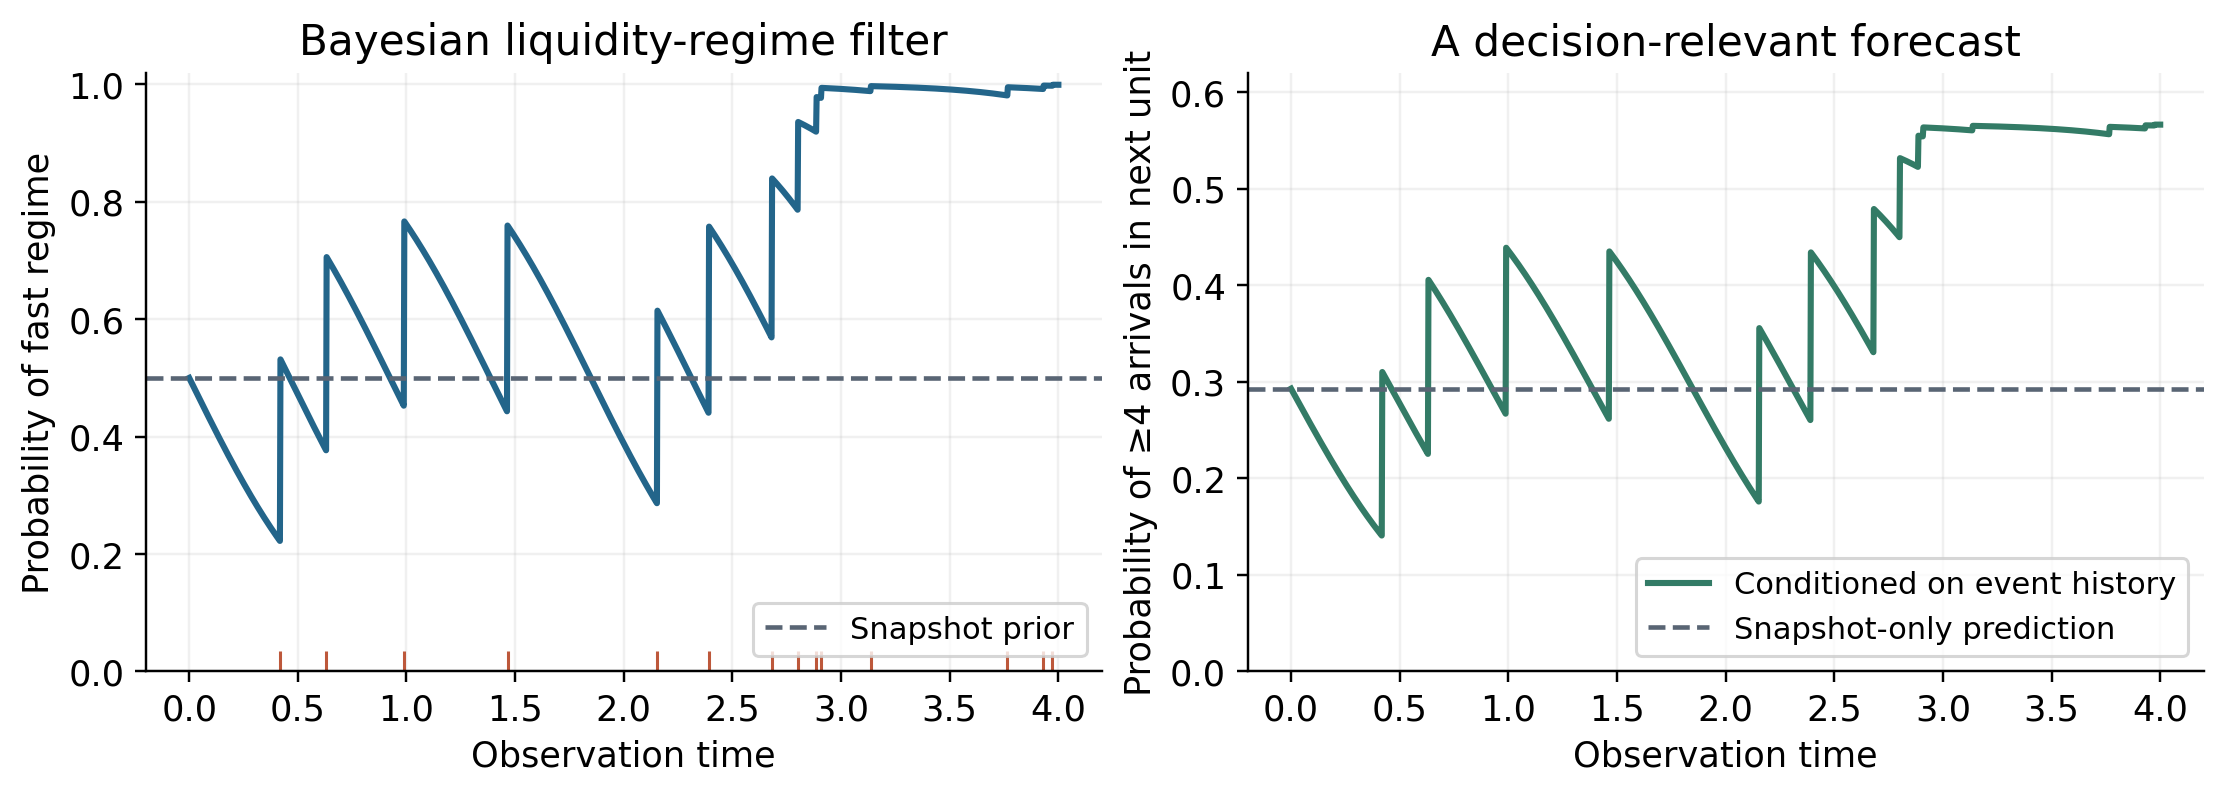
\includegraphics[width=\textwidth]{figures/hidden_liquidity_filter.png}
 \caption{A synthetic fast-regime path and its exact Bayesian filter. Quiet intervals lower the fast-regime probability; arrivals raise it. The right panel shows the resulting forecast for a future arrival-count threshold. The latent regime is not an undepleted hidden reserve.}
 \label{fig:filter}
\end{figure}

\subsection{Exact queue depletion and a path-law certificate}
The second experiment is a continuous-time Markov chain on queue states
$\{0,1,\ldots,6\}$, with state $0$ absorbing. At state $n>0$, the death rate is
$d(n)=1+0.25n$; the birth rate is $1.2$ if $n<6$ and zero at capacity.
The initial state is $4$ and the horizon is $T=2$.
The learned model replaces $d(n)$ by $(1+\theta)d(n)$, leaving births unchanged.

Let $Q$ be the true generator, using row-vector distributions.
Matrix exponentiation gives
$p_T=e_4^\top e^{TQ}$ and the corresponding learned distribution.
The mean-integrated discrepancy is
\begin{equation}
 \E\int_0^T\delta_t\dd t
 =\theta\,e_4^\top\left(\int_0^Te^{tQ}\dd t\right)d
 =3.5212578021\,\theta.
\end{equation}
We evaluate the integral as the upper-right block of
$\exp\bigl(T\left[\begin{smallmatrix}Q&I\\0&0\end{smallmatrix}\right]\bigr)$,
which avoids inverting the singular generator.
The true depletion probability is $0.1693829524$.

\begin{table}[htbp]
 \centering\small
 \begin{tabular}{rrrrrr}
\toprule
$\theta$ & Depl. bias & Terminal TV & $L^1$ bound & KL bound & $|\Delta$CVaR$_{.99}|/B$ \\
\midrule
0.001 & 0.00043 & 0.00061 & 0.00352 & 0.00094 & 0.09379 \\
0.002 & 0.00086 & 0.00122 & 0.00704 & 0.00188 & 0.18753 \\
0.010 & 0.00432 & 0.00611 & 0.03521 & 0.00935 & 0.93514 \\
0.025 & 0.01088 & 0.01522 & 0.08803 & 0.02326 & 1.00000 \\
0.050 & 0.02200 & 0.03024 & 0.17606 & 0.04615 & 1.00000 \\
0.100 & 0.04491 & 0.05962 & 0.35213 & 0.09087 & 1.00000 \\
0.200 & 0.09291 & 0.11544 & 0.70425 & 0.17642 & 1.00000 \\
\bottomrule
\end{tabular}

 \caption{Exact finite-state calculations up to matrix-exponential precision. Depletion bias and terminal TV are measured distributional errors. The $L^1$ and KL columns are full-path TV upper bounds. The final column bounds the absolute CVaR difference divided by cost range $B$, using the smallest available path bound.}
 \label{tab:queue}
\end{table}

At $\theta=0.10$, the depletion probability changes by $0.044909$, terminal TV is $0.059619$, and the mean path bound is $0.352126$. The certificate is conservative but valid. At $\theta=0.20$, the deterministic-envelope bound $0.632121$ is smaller than the mean-integrated bound $0.704252$; either can be used.
For this multiplicative perturbation the exact path KL divergence is
\[
 D_{\rm KL}(P\|\widehat P)=3.5212578021\,[\theta-\log(1+\theta)].
\]
At $\theta=0.10$, Pinsker therefore gives $0.09087$, substantially below the $L^1$ bound while still above terminal TV. At $\theta=0.001$, its 99-percent CVaR error bound is $0.09379B$; at $0.002$, it is $0.18753B$. With the original $L^1$ route alone, a nontrivial 99-percent bound requires $\theta<0.002839894$. The added small-error regimes and likelihood comparison make the informative and vacuous ranges explicit. None of these upper bounds is measured full-path TV.

\subsection{Posterior resolution and a persistent fitting floor}
Take $\mathsf H=L^2(0,1)$ with an orthonormal basis $(e_j)_{j\ge1}$ and target field
\[
 Z=\sum_{j\ge1}\frac{\xi_j}{j}e_j,\qquad \xi_j\stackrel{\rm iid}{\sim}N(0,1).
\]
The learned level-$m$ field has independent coefficients
$[\beta+(1+\eta)\xi_j]/j$ for $j\le m$ and zero coefficients above $m$.
Set $\beta=0.04$ and $\eta=0.06$. Since the covariance operators are diagonal in the same basis, the exact Gaussian Wasserstein error is
\begin{equation}\label{eq:gaussian-posterior}
 \kappa_m^2=\sum_{j>m}j^{-2}
 +(\beta^2+\eta^2)\sum_{j=1}^mj^{-2}.
\end{equation}
This is also the context-independent refinement certificate with $L_j=0$.
For the illustrative density $f_z(u)=1.2+0.4\tanh z(u)$, positivity and
$K=0.4$ hold on $L^2(0,1)$ and $M=1$.
The local posterior-induced rate-error bound is therefore $0.4\kappa_m$.

At $m=256$, $\kappa_m=0.111499$ and the local rate bound is $0.044600$.
The limiting posterior error is $0.092486$, because finer resolution does not remove the bias and variance mismatch in retained coordinates.
This calculation concerns one conditional posterior and its local rate map. Extending it to a complete market path requires the predictable-history assumptions of \Cref{cor:combined}; a one-time Gaussian calculation alone does not establish them.

\begin{figure}[htbp]
 \centering
 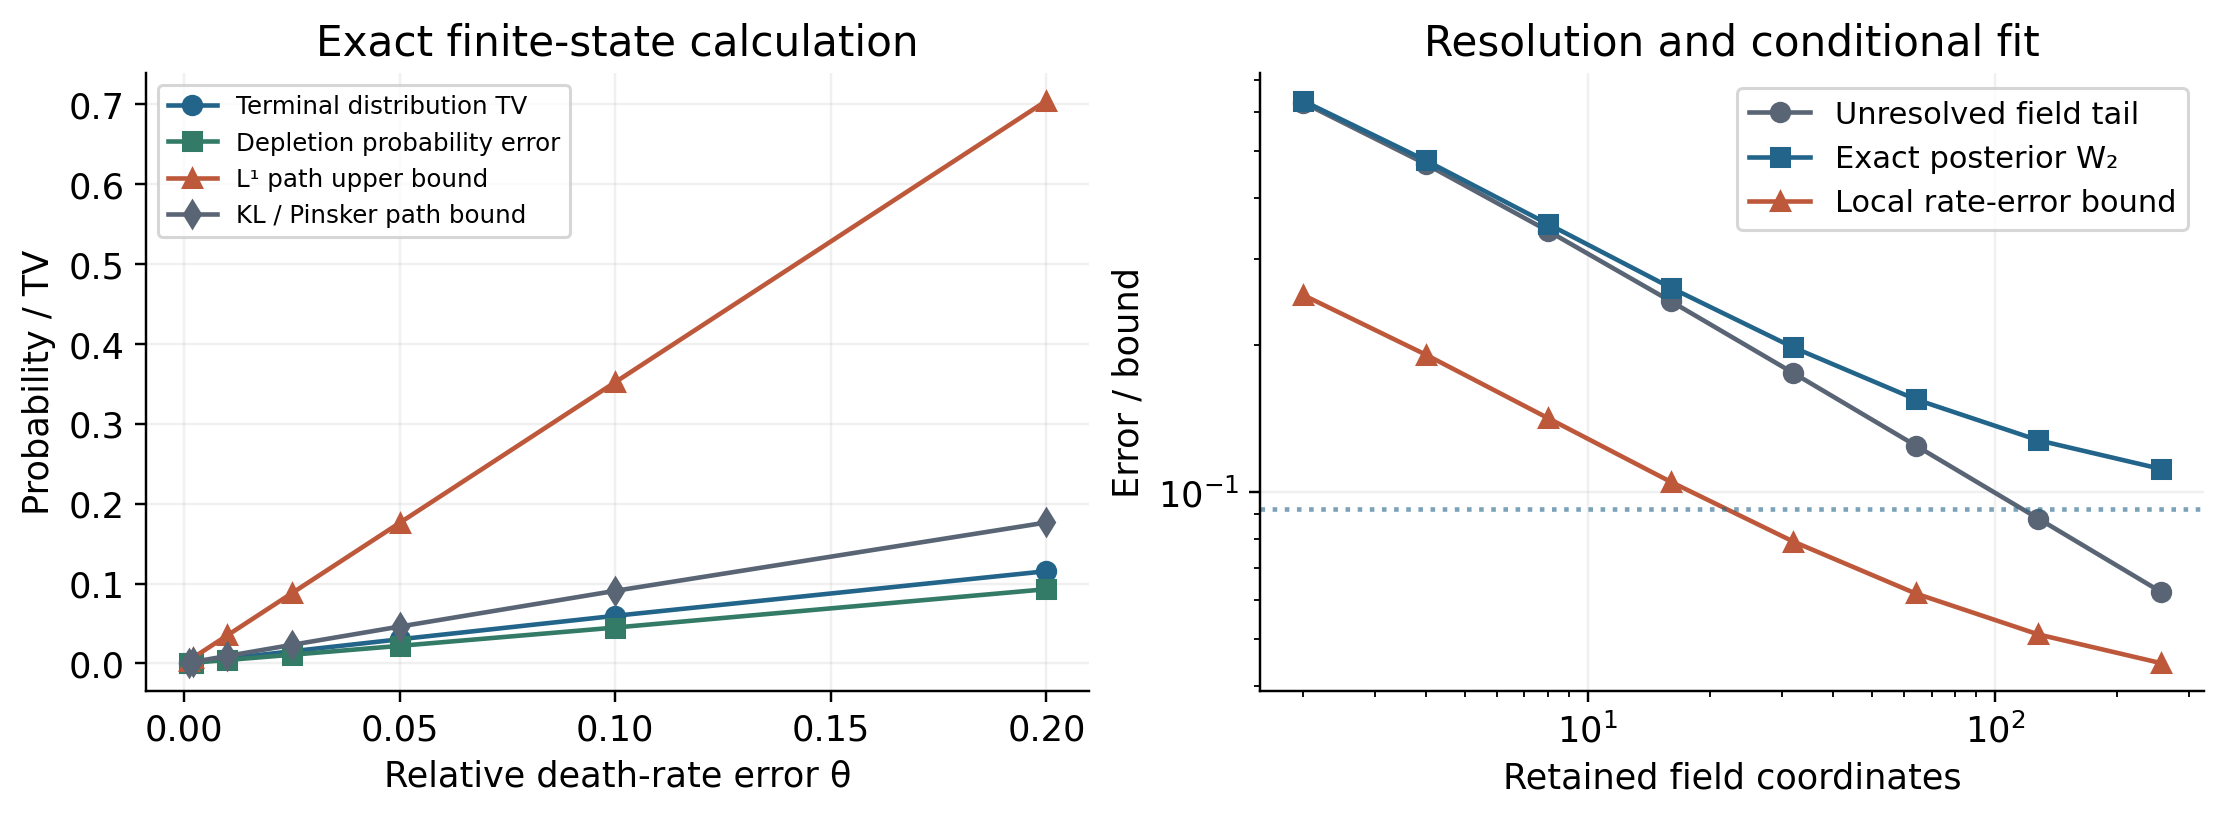
\includegraphics[width=\textwidth]{figures/event_error_certificate.png}
 \caption{Left: exact terminal distribution errors and two full-path upper bounds for the queue chain. Right: the Gaussian posterior calculation \eqref{eq:gaussian-posterior}, its unresolved tail, and the induced local intensity bound. The horizontal dotted line is the persistent posterior fitting floor.}
 \label{fig:certificate}
\end{figure}

\subsection{Liquidity geometry and analytic option prices}
Two static ask books share prices
$(100,100.01,100.03,100.06)$ and have volumes $(2,3,2,3)$ and $(1,2,4,3)$.
Both have ten lots. Their normalized volume transport distance times ten is
$0.05$, exactly the difference between the costs of buying all ten lots.
The partial-quantity costs satisfy \Cref{thm:sweep} at every quantity.

\begin{figure}[htbp]
 \centering
 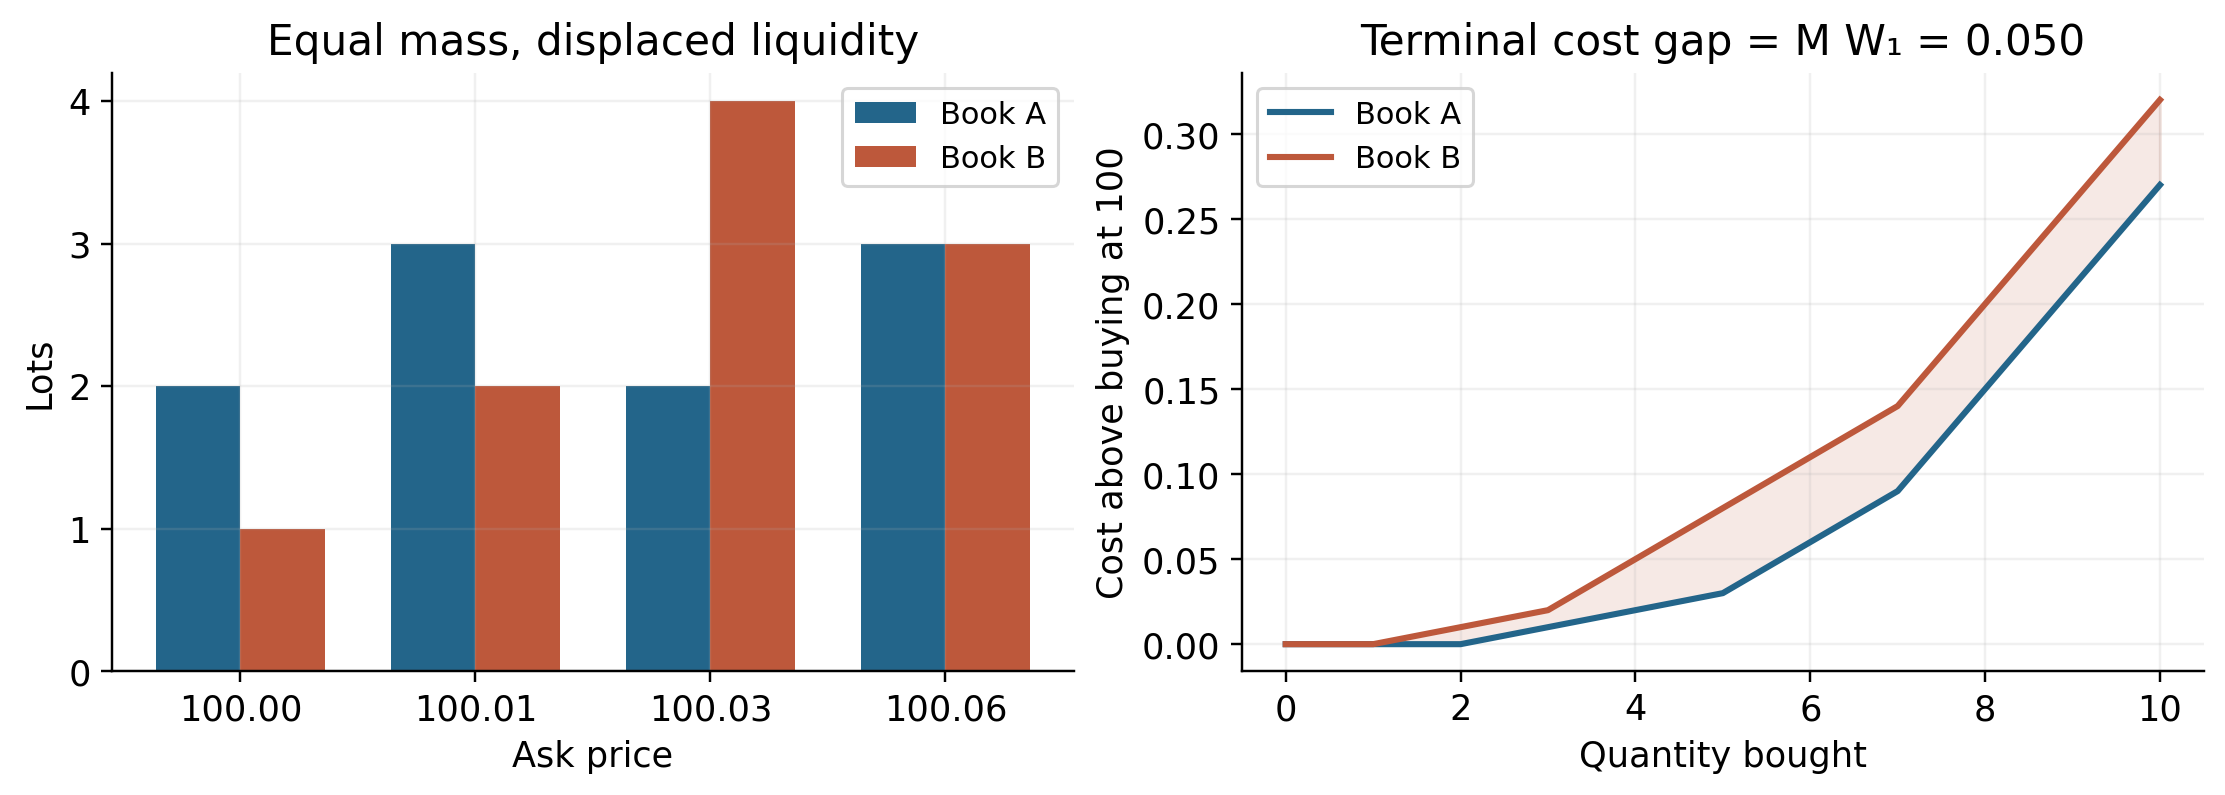
\includegraphics[width=\textwidth]{figures/execution_geometry.png}
 \caption{A sharp static sweep-cost example. The right panel subtracts the common cost $100Q$ to expose the liquidity contribution. The final gap is $0.05$ currency units for ten lots under the stated unit convention.}
 \label{fig:geometry}
\end{figure}

For the pricing illustration, draw a volatility $\sigma\in\{0.15,0.35\}$ with equal probabilities before all return innovations, take $X_0=100$, and use zero interest. Conditional on $\sigma$, use the martingale construction.
Take $\mathcal G_0$ trivial, so the volatility draw is hidden from the market at the pricing origin. The time-zero option price is then the equally weighted mixture of the two analytic lognormal call prices. If the draw is revealed instead, the conditional price is the price for that realized volatility, rather than the mixture.
At-the-money calls at maturities $0.25,0.5,1,2$ have prices
$4.981979$, $7.038809$, $9.935283$, and $13.996948$.
No option-pricing Monte Carlo is needed for these numbers.

\begin{figure}[htbp]
 \centering
 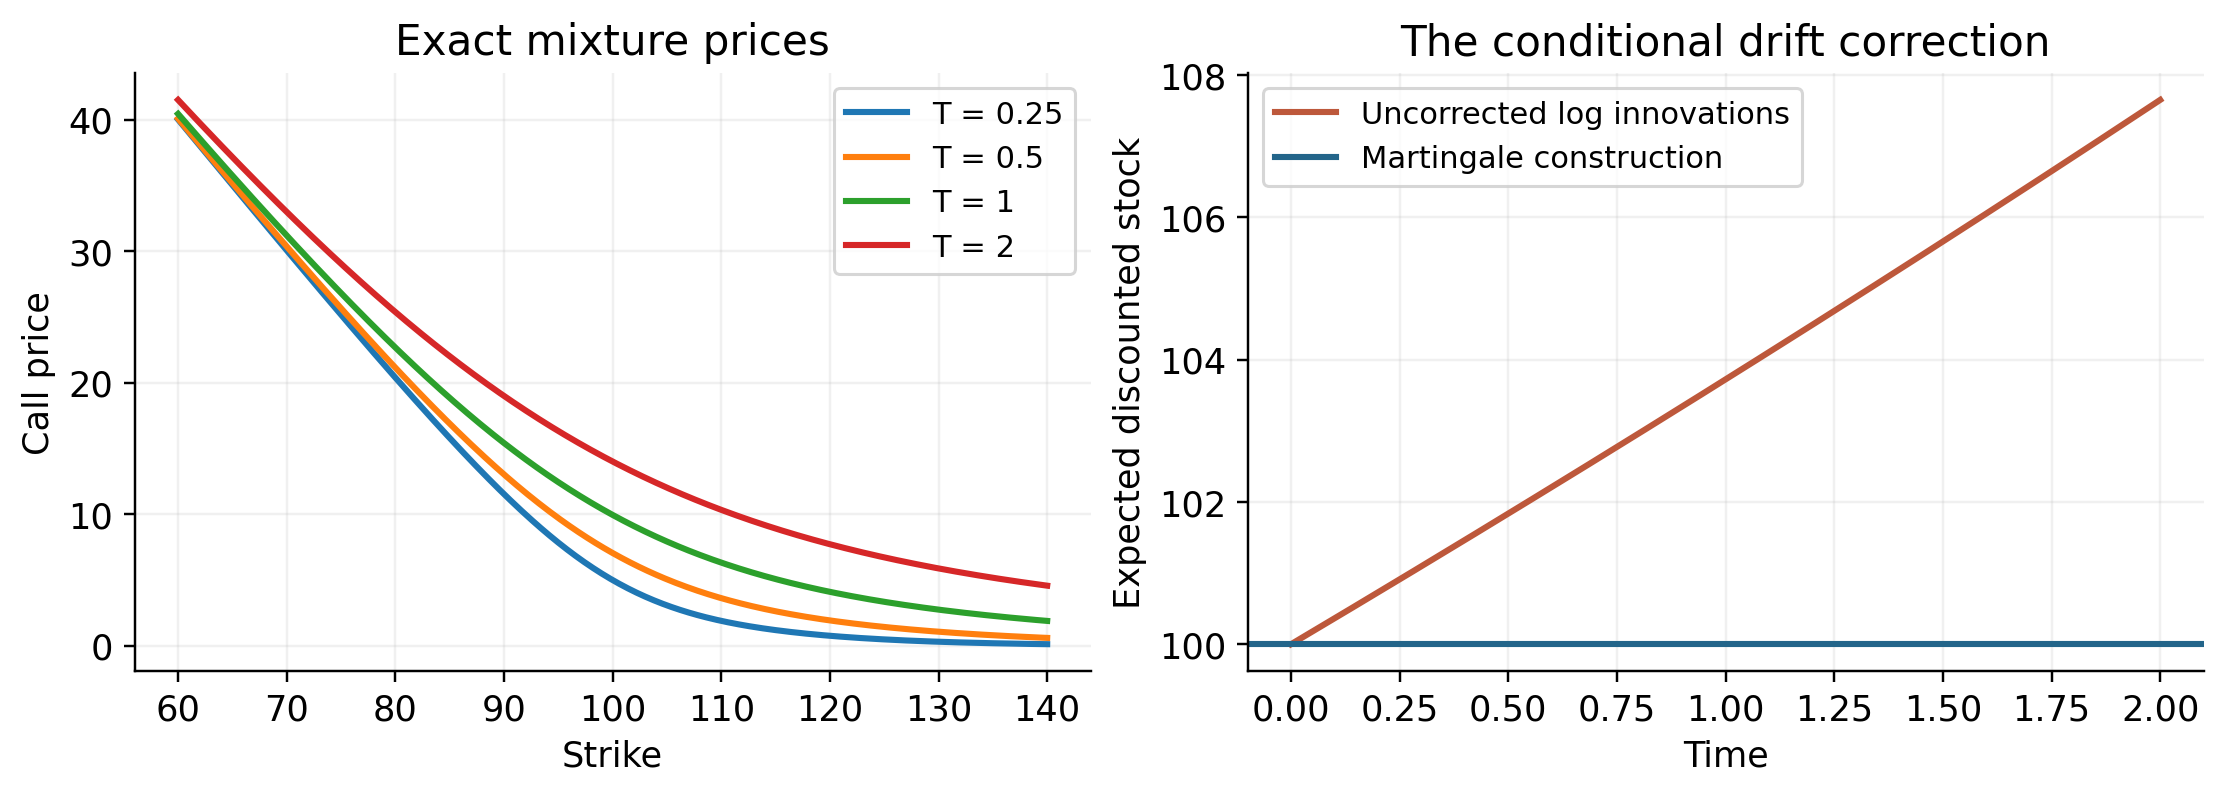
\includegraphics[width=\textwidth]{figures/martingale_pricing.png}
 \caption{A positive mixture martingale with analytic call prices. Omitting the $-\sigma^2T/2$ correction makes the expected discounted stock rise from $100$ to $107.653708$ at $T=2$. Including it keeps that expectation exactly $100$. This is an explicit illustrative generator, not a trained volatility model.}
 \label{fig:pricing}
\end{figure}

\subsection{A complete learned reserve model with an execution decision}\label{sec:complete-model}
This experiment connects hidden inventory, survival-aware filtering, a learned intensity map, exact sampling, and execution evaluation in one model. All rate specifications and labels are synthetic. The model has one displayed ask lot $D=1$, hidden reserve $H\in\{0,\ldots,5\}$, and a fixed hidden regime $R\in\{0,1\}$. Initially $\mathbb P(R=1)=0.4$ and independently $H$ equals $0,2,5$ with probabilities $0.1,0.5,0.4$. This is an explicitly specified aggregate reserve model, not a claim about an exchange's priority rules.

While the trader's passive order is active, the rates are
\begin{equation}\label{eq:complete-rates}
 \lambda_{R,H}=(1+2R)(1+0.08H),\qquad
 \phi_{R,a}=(0.6+0.5a)(0.8+0.4R),\quad a\in\{0,1\}.
\end{equation}
A competing execution consumes the displayed lot. When $H>0$, its mark records a one-lot refresh and updates $(D,H)$ to $(1,H-1)$. When $H=0$, its mark records depletion and the episode ends. An independent passive-fill clock of rate $\phi_{R,a}$ ends the episode with a trader fill. Thus every execution-linked update obeys \eqref{eq:reserve-conservation}. The fill opportunity and its action response are specified parts of this toy market, not inferred counterfactual effects.

The three marks are refresh, depletion, and trader fill. Give each mark a unit-mass event cell; then the conditional rate field is the three-vector
\[
 f(R,H,a)=(\lambda_{R,H}\mathbf1_{\{H>0\}},
          \lambda_{R,H}\mathbf1_{\{H=0\}},\phi_{R,a}),\qquad M=3.
\]
Embed the twelve active hidden states as distinct unit basis vectors in $\R^{12}$. Distinct states are at distance $\sqrt2$. This finite latent geometry accommodates the inventory feasibility indicator directly; no continuous sensitivity is inherited through a discontinuous rounding map.

\paragraph{What is trained.}
A $3$--$24$--$24$--$2$ network with tanh hidden layers and output $10\operatorname{sigmoid}$ receives $(2R-1,H/2.5-1,2a-1)$ and predicts $(\lambda,\phi)$. It has 746 parameters. Training uses all 24 active state/action specifications, with 1,200 Adam updates followed by L-BFGS. The labels are the exact rates in \eqref{eq:complete-rates}; the model is a learned rate emulator, not a market-data estimator. Its finite-domain audit covers every deployed input. This choice isolates whether a learned representation can be inserted into the full probabilistic construction without leaving unmeasured approximation error.

The final mean squared rate error is $4.9514\times10^{-7}$. Exhaustive evaluation gives
\begin{align}\label{eq:complete-constants}
 \epsilon_\lambda&=\max_{R,H,a}\sum_e|f_e-\widehat f_e|=0.00266924,\\
 r_{\max}&=\max_{R,H,a}\|f-\widehat f\|_2=0.00190530,
 \qquad K=3.64972.\notag
\end{align}
Here $K$ is the maximum pairwise learned field difference divided by $\sqrt2$ over required latent states and actions. Both models have total rate below six. The common thinning envelope is therefore $c=6$ on this fully enumerated domain. The analytic bounds are exact mathematical implications; their reported numerical evaluations use float64 and are not interval-arithmetic proofs.

\paragraph{The filter and the decision.}
Before the trader posts, there is no trader-fill clock. For an observed prehistory, the posterior is updated by \eqref{eq:survival-filter}, followed at every refresh by the corresponding likelihood and reserve decrement. We compare three information states: the initial prior; a quiet interval of length $0.5$; and refreshes at $0.1$ and $0.3$ followed by observation through $0.5$. These are specified conditioning histories with positive likelihood density, not selected realized trading records. The neural model uses its own rates to compute its posterior on the same history.

After the two refreshes, the true posterior mean reserve is $1.417759$ and the fast-regime probability is $0.648446$. Dropping survival information gives posterior TV error $0.208696$. The correctly updated neural posterior has TV error $7.97\times10^{-5}$. A direct likelihood calculation over initial states verifies the recursive filter to $5.6\times10^{-17}$.

The trader selects an action $a\in\{0,1\}$ and deadline $\tau\in\{0,0.1,\ldots,1.5\}$. A passive fill costs $0.04a$, depletion before fill costs $1$, and crossing at the deadline while still active costs $0.3$. Costs are per lot in a declared currency unit, with $B=1$. The finite class has 32 configurations and is optimized by enumerating their expected costs. It is a deadline policy class, not the unrestricted solution of a partially observed control problem.

The full model is a 14-state CTMC: twelve active hidden states and two absorbing outcomes. If $p$ is the posterior at the decision origin, $p^Te^{\tau Q_a}$ gives its exact outcome probabilities up to matrix-exponential numerical precision. A neural posterior $\widehat p$ and generator $\widehat Q_a$ give the corresponding model values. No path Monte Carlo is used to choose or value these policies.

\begin{table}[htbp]
\centering\small
\begin{tabular}{lrrrrr}
\toprule
History & Action & Deadline & True cost & Max. value error & Path bound \\
\midrule
initial & 1 & 1.5 & 0.244577 & 1.75e-05 & 4.00e-03 \\
quiet & 1 & 1.5 & 0.223617 & 2.99e-05 & 4.06e-03 \\
two refreshes & 0 & 0.0 & 0.300000 & 7.50e-05 & 4.08e-03 \\
\bottomrule
\end{tabular}

\caption{Exact finite-state policy evaluation. The maximum value error is over all 32 policies at the stated history. The final column is a uniform full-path certificate for the entire deadline class; it is not measured path TV.}\label{tab:complete-model}
\end{table}

Write $\delta_0=\TV(p,\widehat p)$. Couple these initial hidden states maximally and then apply common-event thinning. For every policy in the class,
\begin{equation}\label{eq:complete-path}
 \TV(P^a,\widehat P^a)\le
 1-(1-\delta_0)e^{-1.5\epsilon_\lambda}.
\end{equation}
This gives the final column of \Cref{tab:complete-model}. The same argument bounds the joint hidden-state/history laws at each earlier time, so \Cref{prop:filter-stability} and the $W_1$ version of \Cref{lem:posterior} also give the separate field/posterior certificate
\begin{equation}\label{eq:complete-field}
 \sqrt3\left[1.5r_{\max}
 +2\sqrt2K\int_0^{1.5}\{1-(1-\delta_0)e^{-\epsilon_\lambda t}\}\dd t\right].
\end{equation}
Its values are $0.05857$, $0.06021$, and $0.06070$. The direct full-state coupling is substantially tighter in this small enumerated model. Reporting both shows the price of the representation-level decomposition; it does not conceal it behind the abstract theorem.

The learned and true models select the same policy in each information state, giving zero regret within the enumerated class. After the prior or quiet history, action $1$ with deadline $1.5$ is preferred; after two refreshes, immediate crossing is preferred. The uniform regret bounds are about $0.0080$--$0.0082$ currency units. The corresponding 99-percent CVaR error bounds are $0.3996$--$0.4075$ units, below the trivial bound $B=1$. Several actual policies have CVaR equal to the worst cost; a nontrivial bound is not evidence that their tail losses are small.

\paragraph{Sampling independently checked.}
We implement both exact averaging and one fresh posterior draw per proposal, updating the entire belief after accepted marks. In 20,000 paths for each method, with action $1$, horizon $0.8$, and the two-refresh posterior, all three terminal probabilities agree with matrix exponentiation within five binomial standard errors. Maximum absolute discrepancies are $0.00356$ and $0.00739$. These are sampling diagnostics; exactness of the construction follows from \Cref{prop:posterior-thinning}.

\begin{figure}[htbp]
\centering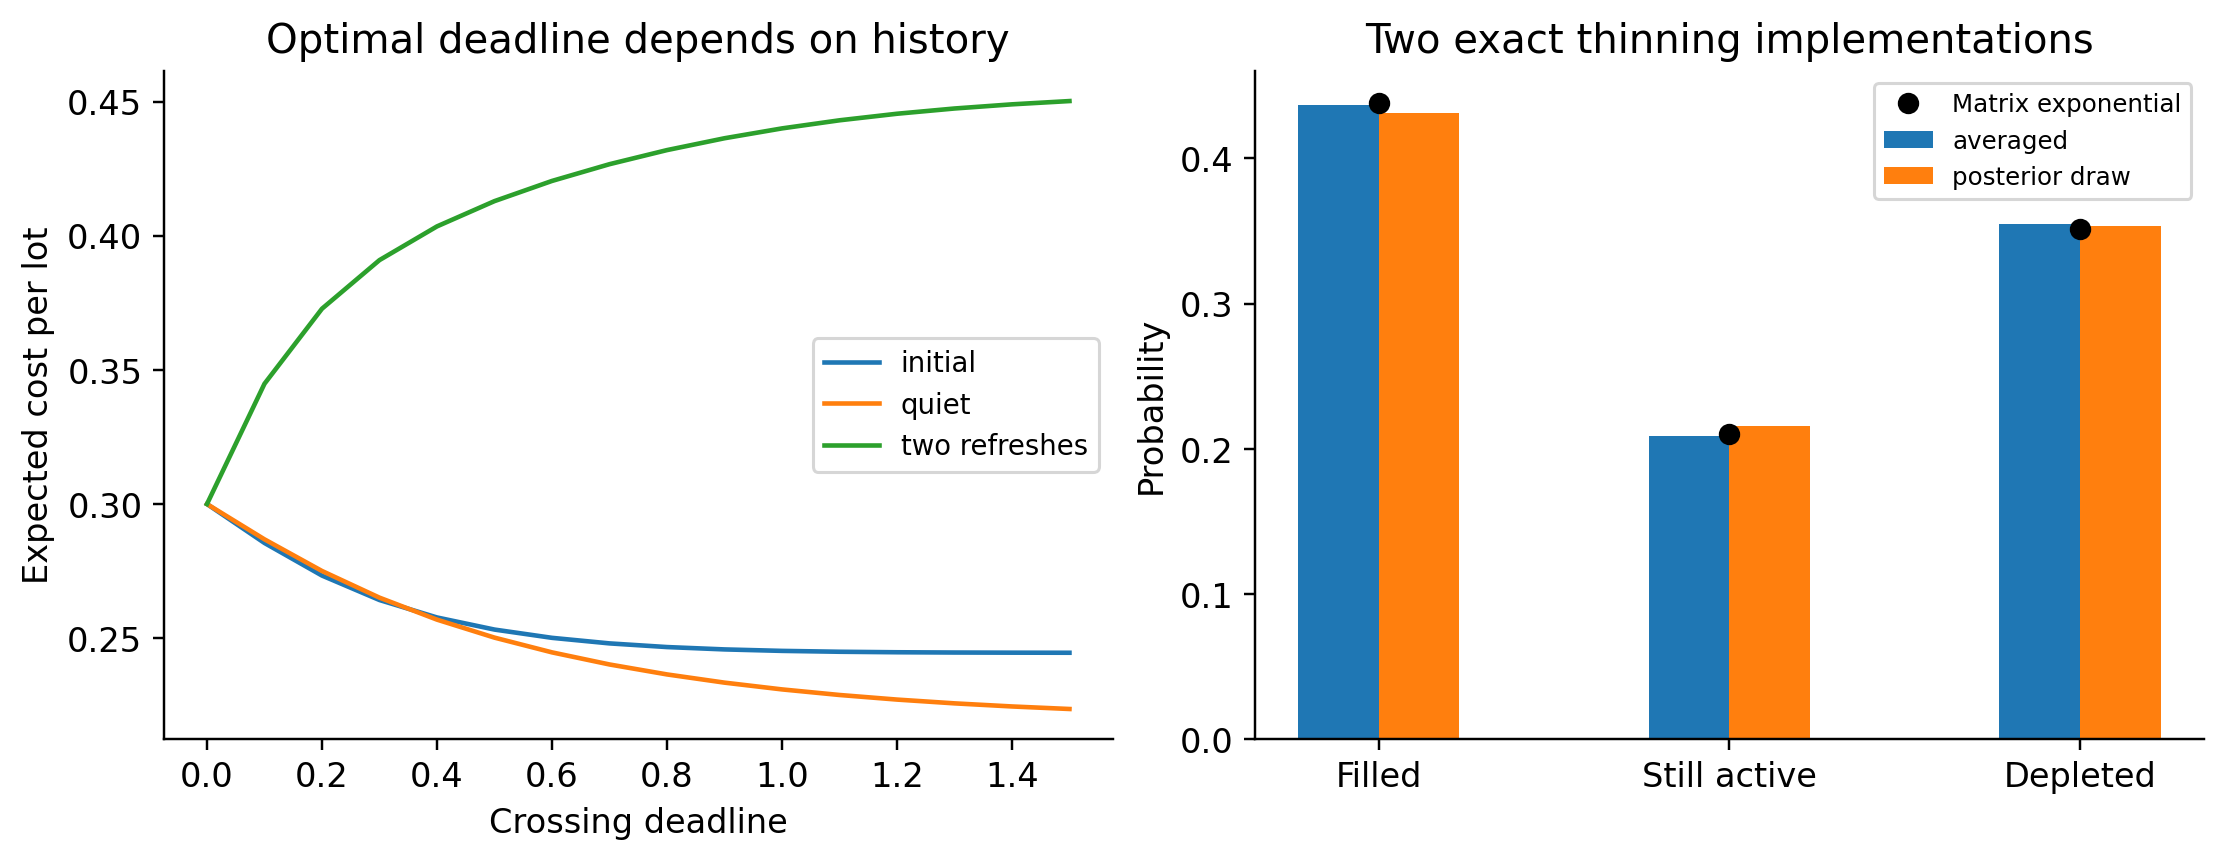
\includegraphics[width=\textwidth]{figures/learned_reserve.png}
\caption{Left: true expected execution cost, minimized over the two action choices at each deadline, for three observed histories. Right: two thinning implementations compared with independently computed CTMC outcome probabilities.}\label{fig:complete-model}
\end{figure}

\subsection{A genuinely adapted volatility perturbation}
To test \Cref{thm:vol-price}, use 32 equal steps over $T=1$ and let
\[
 W_n=\sum_{k<n}\sqrt{\Delta_k}Z_{k+1},\qquad
 \sigma_n=0.2+0.1\tanh(W_n),\qquad
 \widehat\sigma_n=\sigma_n+\delta.
\]
Both volatilities are selected before the next return innovation. For
$\delta\in\{0.005,0.01,0.02\}$, take the common bound $\bar\sigma=0.32$.
The theorem input is exactly $\mathcal A_N=\delta^2$, not an estimated future-path transport distance. From 200,000 common-innovation paths with $X_0=100$, the at-the-money call differences are $0.199253$, $0.398629$, and $0.797714$, with standard errors $0.000892$, $0.001789$, and $0.003602$. The improved deterministic bounds are $0.694672$, $1.389344$, and $2.778688$. Estimated absolute terminal coupling errors are $0.400444$, $0.800891$, and $1.601781$. The bound controls these coupled constructions and Lipschitz payoffs; it is not an assertion that this coupling realizes $W_1$.

\subsection{Learning from event counts and selecting a certified policy}
The reserve experiment tests the partially observed simulator with a specified latent model. A separate finite observable example tests the statistical and control results of \Cref{sec:certified-control} using event data alone. Its role is to isolate what can be certified when state-action exposure is actually observed.

The state is $(q,z)$ with remaining quantity $q\in\{0,1,2,3,4\}$ and observed regime $z\in\{0,1\}$. The actions are passive ($a=0$) and aggressive ($a=1$). A fill reduces $q$ by one; a regime mark changes $z$ to $1-z$. States with $q=0$ are absorbing. For positive quantity the synthetic rates are
\begin{align}\label{eq:control-truth}
 \lambda_{\rm fill}(q,z,a)&=(0.75+0.10q)(1+0.35z)(1+1.8a),\\
 \lambda_{\rm regime}(q,z,a)&=0.35+0.10q+0.12a+0.20z.\notag
\end{align}
Their known envelopes are $5$ and $1.5$. At horizon $T=2$, the terminal cost is $q(1+0.2z)$; running cost is $0.03q^2$; a passive fill costs $0.03$ and an aggressive fill costs $0.35$. Regime changes have no direct cost. This fully specified objective measures an execution trade-off, without purporting to reproduce an exchange fee schedule or empirical spread process.

Each observed episode starts with randomized positive quantity and regime. A behavior action is chosen independently at the initial state and after each event, and held until the next event or horizon. The recorded sufficient statistics are the event counts and occupation times for every state-action-mark triple. Three independent streams use seeds $5101,5102,5103$ and prefixes of $2{,}000$, $8{,}000$, and $32{,}000$ episodes. The rate intervals use sixteen geometrically spaced positive $\eta$ values between $0.005$ and $1$, with the 1\% failure budget divided across the three streams. Time-uniform coverage includes every prefix without an additional prefix penalty. The 32 active triples, confidence endpoints, exposures, and counts are serialized.

A $3\to12\to2$ tanh network with sigmoid rate outputs has 74 parameters. Its inputs encode quantity, regime, and action, and its output envelopes are the known rate caps. Training uses $1{,}400$ Adam steps on the exposure-weighted negative log-likelihood
$\sum_i\{\widehat\lambda_i E_i-N_i\log\widehat\lambda_i\}$.
The true rates in \eqref{eq:control-truth} are never training labels. The deployed rate vector is clipped to the confidence box, with the raw network output also retained. The nominal neural policy minimizes its estimated cost. The robust policy minimizes the upper Hamiltonian over the whole box; its guarantee does not depend on successful network optimization. This separation makes it possible to assess both learned predictions and uncertainty-aware decisions.

Both robust equations use $8{,}000$ time steps and the residual allowance in \Cref{prop:control-residual}. The true costs of the resulting feedback policies are computed by matrix exponentiation over runs of identical action vectors. This evaluates the actual continuous-time policy, including possible changes of action at grid boundaries. A high-accuracy DOP853 solution computes the known-model optimum, independently cross-checked against a $16{,}000$-step Euler solution and its residual allowance. Truth enters these diagnostics, not the data-derived confidence box or robust decision.

\begin{table}[htbp]
\centering\small
\begin{tabular}{rrrrr}
\toprule
Episodes & Neural regret & Robust regret & 99\% regret bound & Time residual \\
\midrule
2,000 & 0.00214 & 0.02138 & 1.0618 & 0.0104 \\
8,000 & 0.00014 & 0.00657 & 0.4681 & 0.0105 \\
32,000 & 0.00004 & 0.00161 & 0.2341 & 0.0102 \\
\bottomrule
\end{tabular}

\caption{Execution from initial state $(4,0)$. The neural and robust regrets are means over the three fixed data streams, evaluated against the known synthetic optimum. The confidence column is the largest theorem-derived bound across those streams, including time discretization; the final column is the largest sum of numerical residual allowances. Confidence refers to the analytic event, not a formally rounded floating-point enclosure.}\label{tab:certified-control}
\end{table}

The known optimum is $1.733392$. At $32{,}000$ episodes, robust-policy regret ranges from $0.001178$ to $0.001968$, while its certificate ranges from $0.226235$ to $0.234137$. All true rates fall inside their intervals in the reported runs; this observed coverage is a diagnostic, not a substitute for the simultaneous theorem. The nominal neural policy has lower realized regret in these examples. Robustness therefore has a measured conservatism cost; these experiments do not claim that pessimism always improves realized performance. Rectangular uncertainty and protection against every admissible rate vector explain part of the gap between measured regret and its bound.

\begin{figure}[htbp]
\centering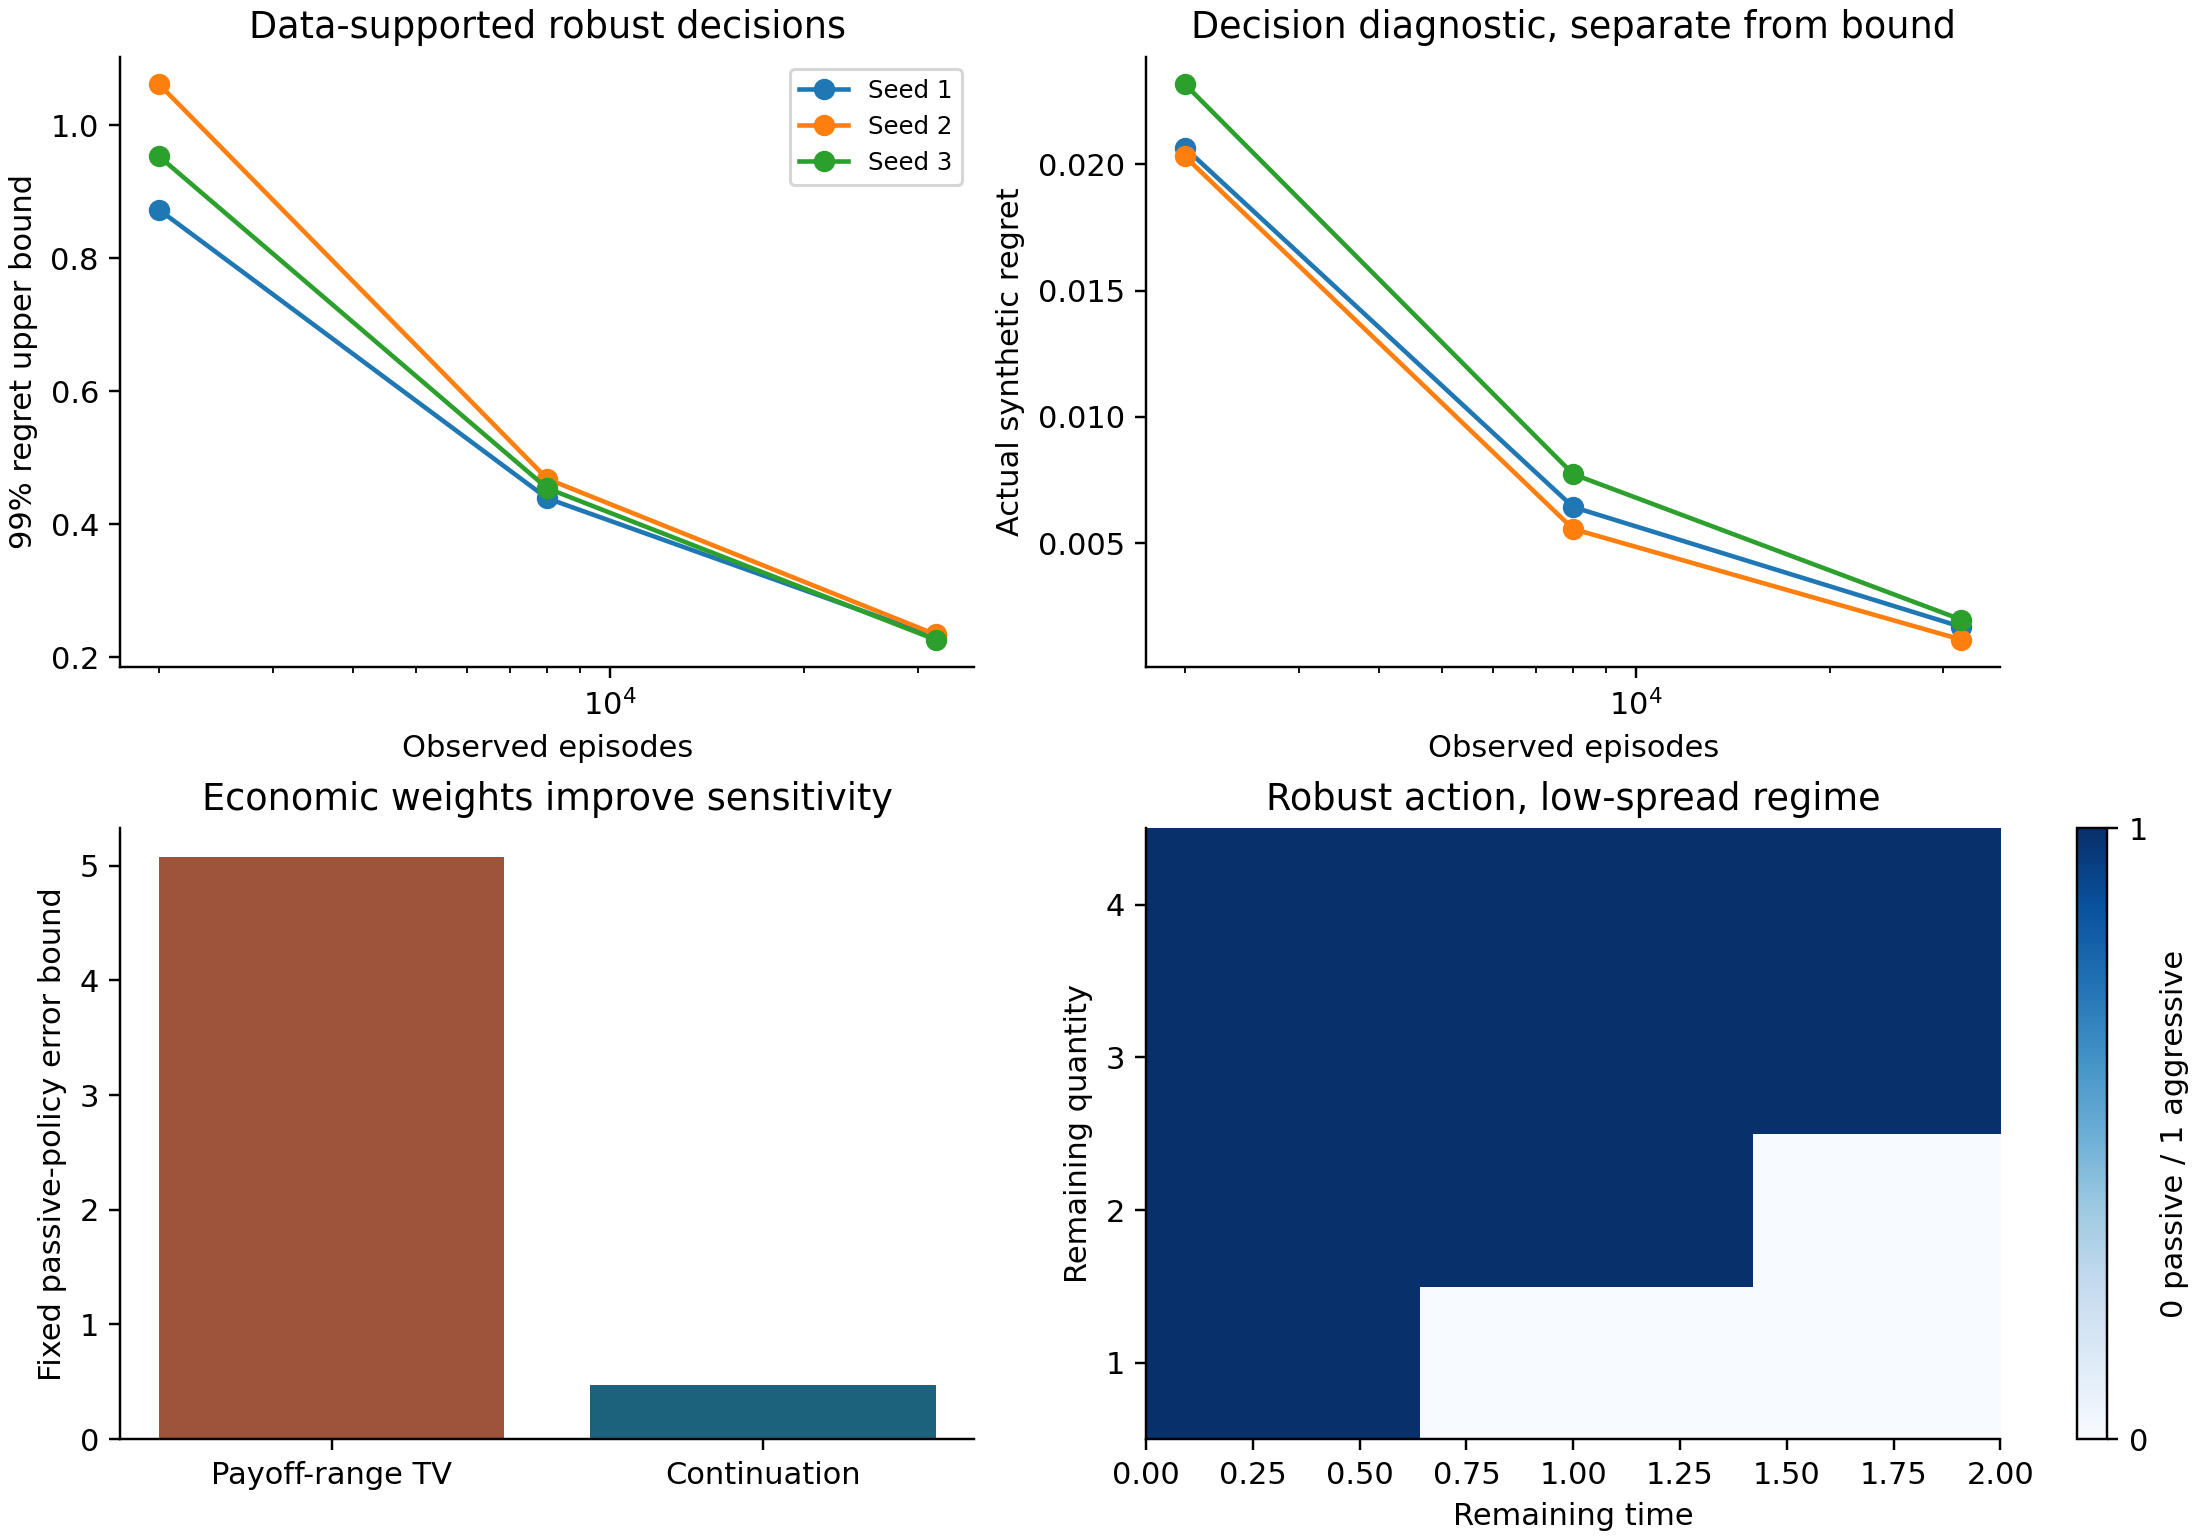
\includegraphics[width=\textwidth]{figures/certified_control.png}
\caption{Observed-event learning and decision certification. Upper panels separate the simultaneous regret bound from actual synthetic regret. Lower left compares two uncertainty bounds for a fixed passive policy. Lower right shows the robust feedback action at the largest data budget of the first stream.}\label{fig:certified-control}
\end{figure}

\subsection{Sensitivity and numerical error in the same decision model}
For the fixed passive policy in the first stream's largest dataset, the exact true-minus-learned cost difference is $-0.00904582$. Numerical integration of the signed continuation identity differs by only $4.82\times10^{-9}$. The statewise continuation bound is $0.469600$, compared with $5.071310$ from the payoff-range times path-TV route using the same rate intervals. Their ratio is about $10.80$. The comparison is objective-specific; a different payoff can assign very different weights to the same events. The continuation integral is numerically evaluated on 2,001 time points and is not claimed to have a rigorous quadrature enclosure.

Doubling the upper-control grid from $8{,}000$ to $16{,}000$ steps changes its initial value by $7.32\times10^{-5}$. The corresponding analytic residual allowances are $0.004900$ and $0.002450$. This check supports the implementation and expected first-order refinement. The allowance bounds the continuous-time interpolation error in exact arithmetic; the program labels its floating-point results accordingly.

Finally, the equal-terminal-law example in \Cref{ex:early-information}, evaluated at $r=0.1$, has early-revelation American value $0.452419$ and late-revelation value $0.409365$. The European values coincide at $0.409365$. The calculation isolates information timing, which neither terminal-law calibration nor an arbitrary path coupling can remove.


\subsection{Reproducibility and limits of the calculations}
The initial Python program regenerates four PNG figures, the queue table, and its JSON results. The reserve and observed-control programs add their respective figures, tables, learned parameters, and full diagnostic records. Each program records its seeds and software versions. It checks the filter against an independent Bayes calculation; generator row sums and integrated occupation time; probability and terminal-TV inequalities; the sharp sweep-cost example; call monotonicity and convexity on the reported grid; and reserve conservation and nonnegativity over 784 admissible integer event combinations.

These are useful consistency checks, but they are not proofs of the continuous statements. The Lean project verifies selected universal statements exactly, while the manuscript proves the analytic results. The new reserve experiment trains a rate network on known synthetic specifications, audits every deployed state/action, and compares exact decision values. The other illustrations remain explicit mathematical examples. No exchange-data calibration or investment-performance claim is made.
